%    JJJ    AA     CCCCCC KKK   K TTTTTT HH  HH EEEEEE BBBBBB UU  UU SSSSSS    CCCCCC OOOOOO MM  MM
%    JJJ   AAAA    CCCCCC KKK  K  TTTTTT HH  HH EEEEEE BB   B UU  UU SSS       CCCCCC OOOOOO MM  MM
%    JJJ  AA  AA   CC     KKK K     TT   HHHHHH EEE    BB   B UU  UU SSS       CC     OO  OO MMMMMM
%    JJJ AA    AA  CC     KKKK      TT   HHHHHH EEEEEE BBBBBB UU  UU  SSSSS    CC     OO  OO M MM M
%    JJJ AAAAAAAA  CC     KKK K     TT   HH  HH EEE    BB   B UU  UU    SSS    CC     OO  OO M MM M
% JJJJJJ AA    AA  CCCCCC KKK  K    TT   HH  HH EEEEEE BB   B UUUUUU    SSS .. CCCCCC OOOOOO M MM M
% JJJJJJ AA    AA  CCCCCC KKK   K   TT   HH  HH EEEEEE BBBBBB UUUUUU SSSSSS .. CCCCCC OOOOOO M MM M
% 
% Texte Geschrieben von Stefan Bopp und Chantal Frunz
% Mehr Informationen sind auf jackthebus.com zu finden


\section{Elektrisches System}
\subsection{�bersicht}
Die Batterie sorgt f�r eine von aussen unabh�ngige Stromversorgung im Bus. Es gibt drei verschiedene Arten die Batterie zu laden:

\begin{enumerate}
\item Die Solaranlage 
\item Das Batterieladeger�t (230V)
\item Das Batterie zu Batterieladeger�t
\end{enumerate}

Dieser Aufbau erm�glicht eine kontinuierliche Stromversorgung.
W�hrend dem Fahren wird die Batterie �ber das Batterie zu Batterieladeger�t geladen, auf dem Campinplatz wird mittels 230V die Batterie geladen und sobald die Sonne scheint, l�dt das Solarpanel mit maximum 70 W die Batterie. 
Es sollte also immer gen�gend Strom vorhanden sein.

Auf der Nachfolgenden Seite ist eine �bersicht des elektrischen Systems zu finden.

\nextpage
\begin{figure}[H]
	\centering
  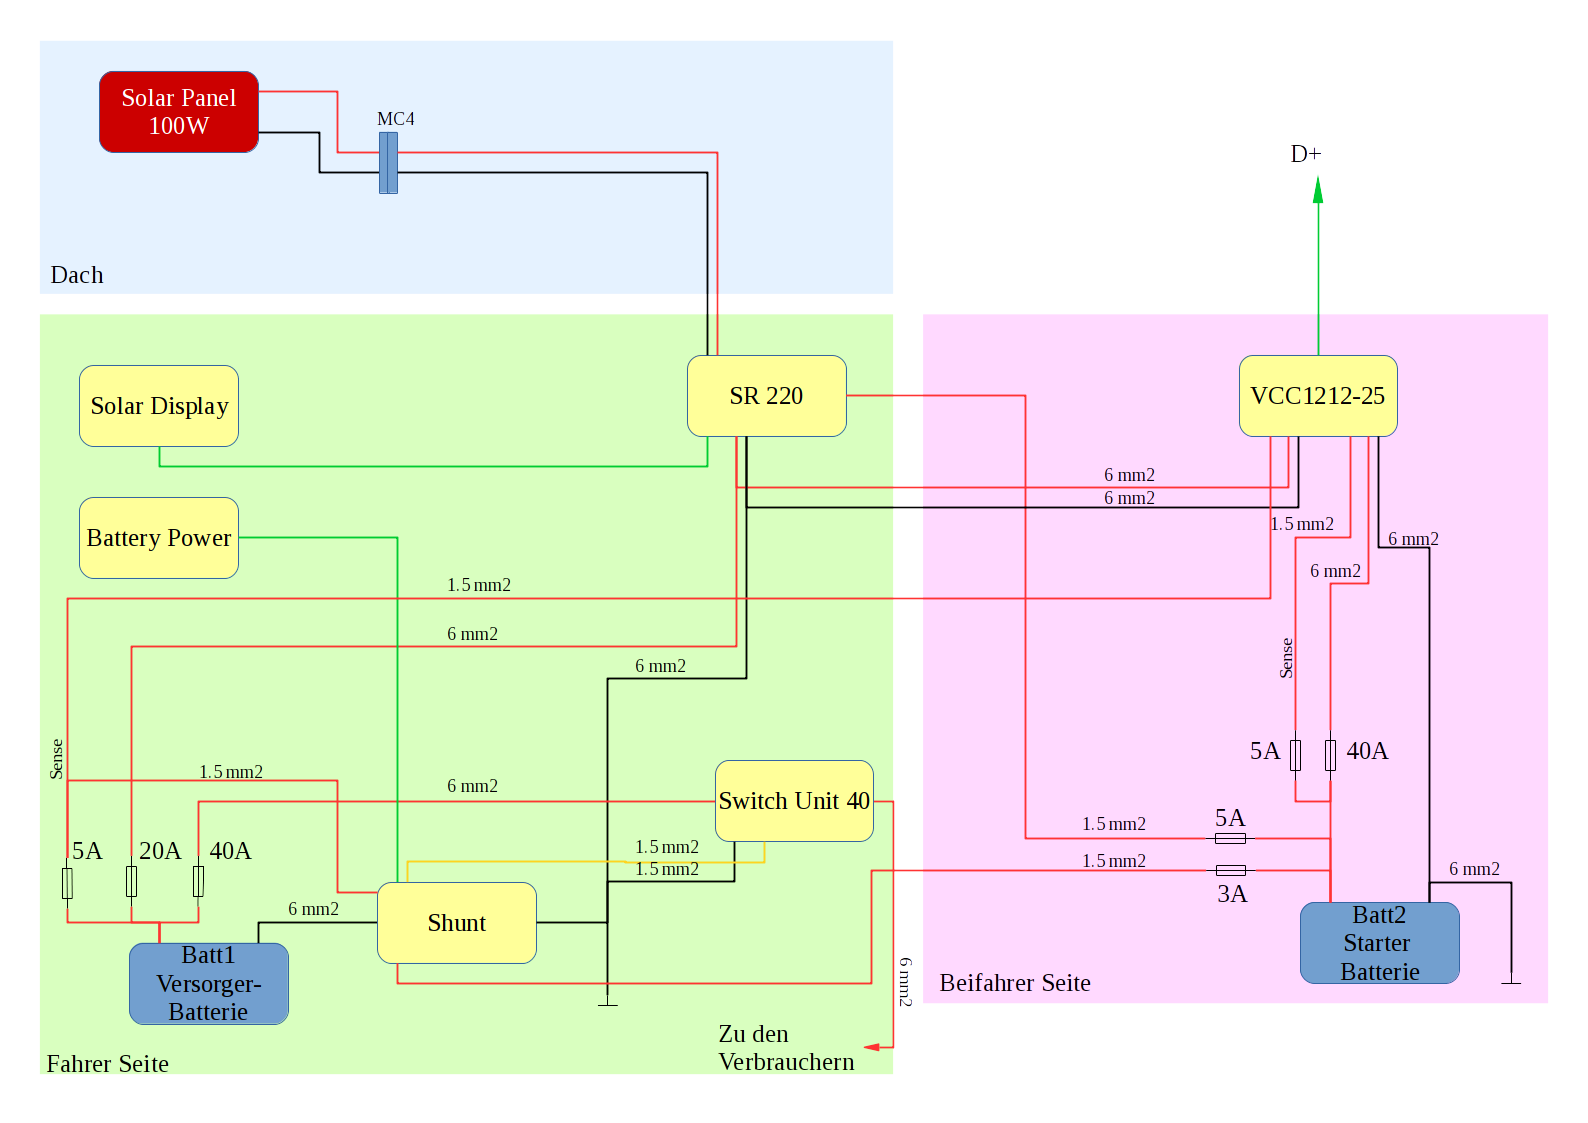
\includegraphics[scale=0.4, angle=90]{../Bilder/Anleitung/EL_System.pdf}
	\caption{�bersicht �ber das elektrische System}
	\label{fig1}
\end{figure}

\subsection{Solaranlage}

Ein 100 Watt Solarpanel auf dem Dach des Busses sorgt f�r die Energieversorgung wenn sonst keine Energiequelle vorhanden ist. 
F�r die Steuerung des Systems ist ein kleines Display in der linken Seitenwand verbaut.
Es dient haupts�chlich zur Anzeige des Status der Anlage.
Einstellungen dar�ber m�ssen keine gemacht werden.
Das System schaltet sich automatisch ab und an, je nach dem Stand der Energiegewinnung
Falls die Batterien voll geladen sind, kann keine zus�tzliche Energie produziert werden.
Dann kann auch bei sch�nstem Wetter die Stromproduktion gegen Null gehen.
Ist somit also kein Fehler der Anlage.
Das zweite Display zeigt den Ladezustand der Batterie an und kann somit zur Pr�fung dienen.

\subsection{Batterie Management}
\subsection{Batterie zu Batterie Ladeger�t}
\subsection{230V zu Batterie}
\subsection{Inverter}
\subsection{USB Anschluss}
\subsection{Licht}
\subsection{Sicherungen}
\subsection{Ersatzsicherungen}
\section{Standheizung}
\subsection{Heizen}
\subsection{L�ften}
\section{K�hltruhe}
\section{Wasser}
\subsection{Wasserpumpe}
\subsection{Abwasser}
\subsection{Frischwasser Kanister}
\section{Kochen}
\subsection{K�chenutensilien}
\section{Radio}
\subsection{Mit eingeschalteter Z�ndung}
\subsection{Betrieb ohne Z�ndung}
\section{Pneu Wechsel}
\subsection{Anzugsmomente}
\subsection{Ludtdruck}
\section{Aufstelldach}
\section{Markise}
\section{Paulchen}
\section{Ordner mit allen Unterlagen}
\section{Ersatzteile}
\section{Werkzeug}
\section{Versicherung}
\section{TCS}


